
\section{图形}
\thispagestyle{fancy}
\LaTeX2e 插图指南手册见 \ref{texref}

[htbp]选项用来指定插图排版的理想位置,这几个字母分别代表here、top、bottom、floatpage,也就是固定位置、页顶、页尾、单独的浮动页。我们可以使用这几个字母的任意组合,一般不推荐单独使用 [h]。\\

%%%%%%%%%%%%%%%%%%%%%%%%%%%%%%%%%%%%%%%%%%%%%%%%%%%%%%%%%%%%


\subsection{插图宏包 graphicx宏包}
在导言区加入下列代码可指定图片存放路径。
 \graphicspath{{figures/}}
\index{宏包!graphicx}
\index{命令!\verb$\includegraphics$}

 可以执行旋转,缩放,指定宽度,裁减。

\begin{lstlisting}[language={[LaTeX]TeX}]
\begin{figure}[htbp]%`位置选项`
\centering
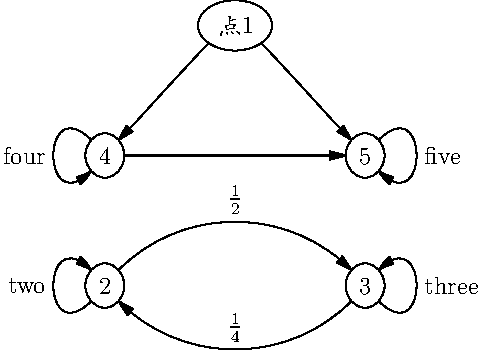
\includegraphics[angle=45,width=9cm]{test1.pdf}
\caption{`测试图片`} \label{test1}
\end{figure}
\end{lstlisting}

\begin{figure}[htbp]%位置选项
\centering
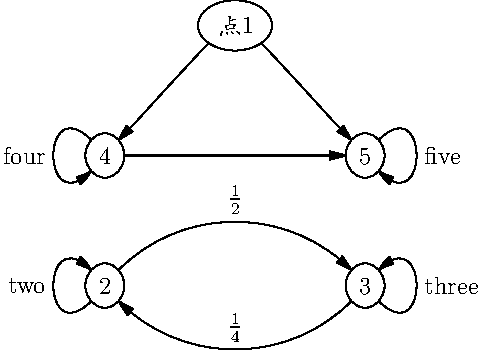
\includegraphics[angle=45,width=9cm]{test1.pdf}
\caption{测试图片} \label{test1}
\end{figure}


%%%%%%%%%%%%%%%%%%%%%%%%%%%%%%%%%%%%%%%%%%%%%%%%%%%%%%%%%%%%

\subsection{并排摆放,一个标题}
两幅图片中间不用换行符就会并排摆放了。
\begin{lstlisting}[language={[LaTeX]TeX}]
\begin{figure}[htbp]
\centering
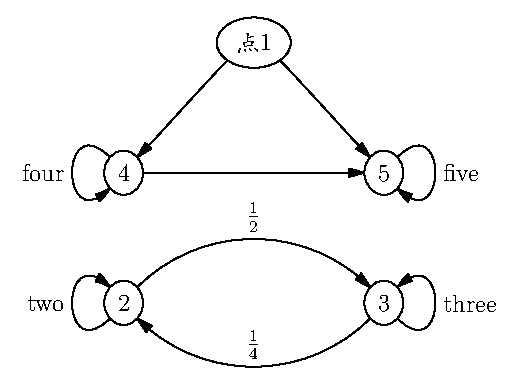
\includegraphics[width=5cm]{test1}
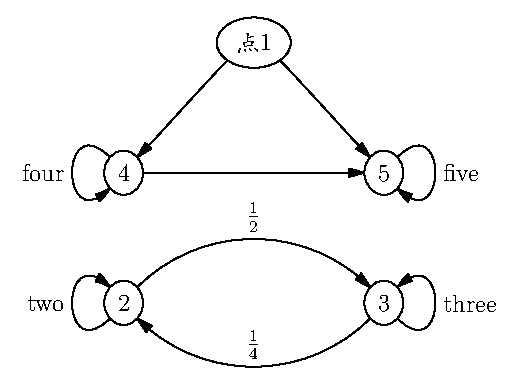
\includegraphics[width=5cm]{test1}
\caption{`并排一个标题`}
\end{figure}
\end{lstlisting}


\begin{figure}[htbp]
\centering
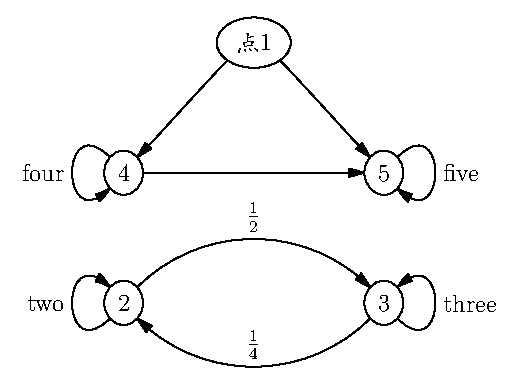
\includegraphics[width=5cm]{test1}
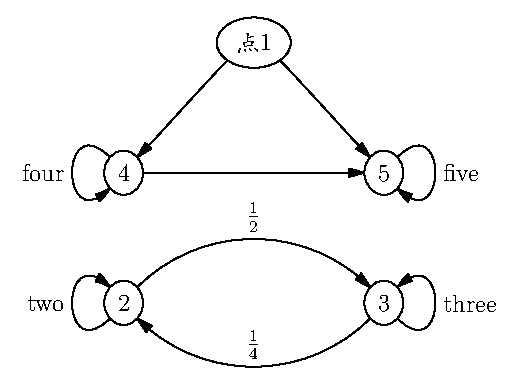
\includegraphics[width=5cm]{test1}
\caption{`并排一个标题`}
\end{figure}


%%%%%%%%%%%%%%%%%%%%%%%%%%%%%%%%%%%%%%%%%%%%%%%%%%%%%%%%%%%%

\subsection{并排摆放,各有标题}
主要是 minipage 环境的使用。
\begin{lstlisting}[language={[LaTeX]TeX}]
\begin{figure}[htbp]
\centering
\begin{minipage}[t]{0.3\textwidth}
\centering
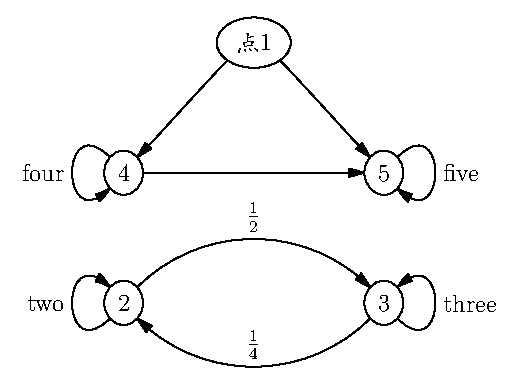
\includegraphics[width=5cm]{test1}
\caption{`左1`}
\end{minipage}
\begin{minipage}[t]{0.3\textwidth}
\centering
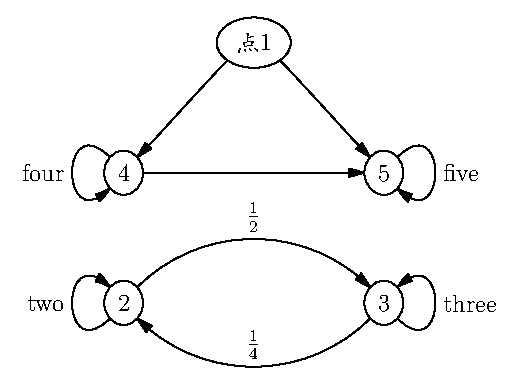
\includegraphics[width=5cm]{test1}
\caption{`左2`}
\end{minipage}
\end{figure}
\end{lstlisting}

\begin{figure}[htbp]
\centering
\begin{minipage}[t]{0.3\textwidth}
\centering
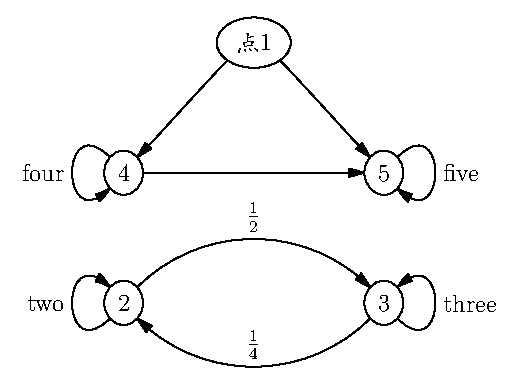
\includegraphics[width=5cm]{test1}
\caption{`左1`}
\end{minipage}
\begin{minipage}[t]{0.3\textwidth}
\centering
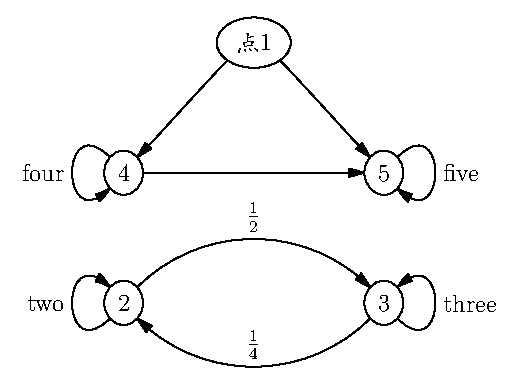
\includegraphics[width=5cm]{test1}
\caption{左2}
\end{minipage}
\end{figure}

\clearpage


%%%%%%%%%%%%%%%%%%%%%%%%%%%%%%%%%%%%%%%%%%%%%%%%%%%%%%%%%%%%

\subsection{图文绕排 picinpar宏包}
此宏包可将图形,表格,文字嵌入到文本中进行排版,提供三种环境 window,figwindow,tabwindow。

\index{命令!\verb$\begin{window}$}
\index{宏包!picinpar}

\begin{lstlisting}[language={[LaTeX]TeX}]

\begin{window}[`行数,列数,对象,`{`标题`}]
  `绕排文本`
\end{window}
\end{lstlisting}
\begin{description}
  \item[行数] 绕排对象上方的文字行数
  \item[列数] l,r,c对象在左,中,右的位置
  \item[对象] 可以为图形,表格,文本
  \item[标题] 对象的标题,如果是 figwindow 或 tabwindow 环境会加上图号和表号
\end{description}


\begin{figwindow}[2,r,{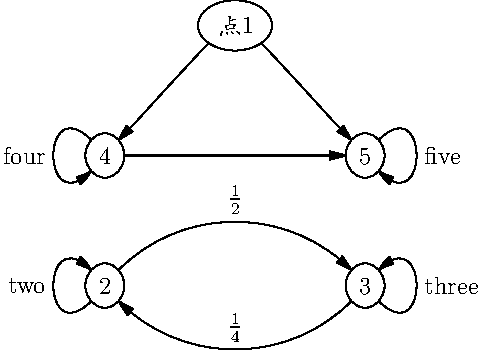
\includegraphics[width=8cm]{test1.pdf}},{绕排}]
平林漠漠烟如织,寒山一带伤心碧。暝色入高楼,有人楼上愁。
玉梯空伫立,宿鸟归飞急。何处是归程,长亭更短亭。泰戈尔
夏天的飞鸟,飞到我的窗前唱歌,又飞去了。秋天的黄叶,它
们没有什么可唱,只叹息一声,飞落在那里。时间可以摧毁世界上的一切,
可以把最坚固的城堡化作历史的残迹,可以把人类的偶像和权威化成灰烬,
可以把英雄的利剑化作孩子的玩物,可以把布满大森林的山脉变成布满珊瑚丛的无边的海洋。
然而,时间也可以造就一切,可以给猿人居住的洞穴变成金碧辉煌的高楼,可以给曾是残破的荒村变成繁华的城市,
也可以使无知的孩子变成百科全书式的学者,在自己的心中展开一个智慧的大星空。
\end{figwindow}


%%%%%%%%%%%%%%%%%%%%%%%%%%%%%%%%%%%%%%%%%%%%%%%%%%%%%%%%%%%%

\subsection{背景水印图片宏包 wallpaper xwatermark}
